\section{Dynamic Obstacles in a GridWorld} 
We first evaluate the performance of our dio/rl implementation compared to an implementation making only use of rl. 
\subsection{Scenario in Reinforcement Learning}
Our autonomous agent exists in an 8x8 grid world. Its goal is to reach the goal from his initial position (1,1).
Along the way, there exists dynamic obstacles which movements is unknown. The agent is punished if colliding with an obstacle and the episode, hereby ends. 
This environment offered by gym-gridworld \cite{gym_minigrid} is useful for testing our algorithm in a Dynamic Obstacle avoidance for a partially observable 
environment. Precisely, we define the state as follows. 
\begin{equation*}
  S_t = [x, y, d, G]
\end{equation*}
$(x,y)$ define the position of our agent while $d$ its direction. $G$ is the gridworld observed by the agent which includes walls, obstacles and free squares. 
The action space is, 
\begin{equation*}
  A_t = \{ right: 0, up: 1, down: 2, left: 3 \}
\end{equation*}
Finally, the reward is a function of the distance from the goal defined as, 
\begin{equation*}
  R_t = 1 - 0.9*(\dfrac{steps}{max\_steps})
\end{equation*}

\medskip

\begin{multicols}{2}
    \begin{figure}[H]
      \centering
      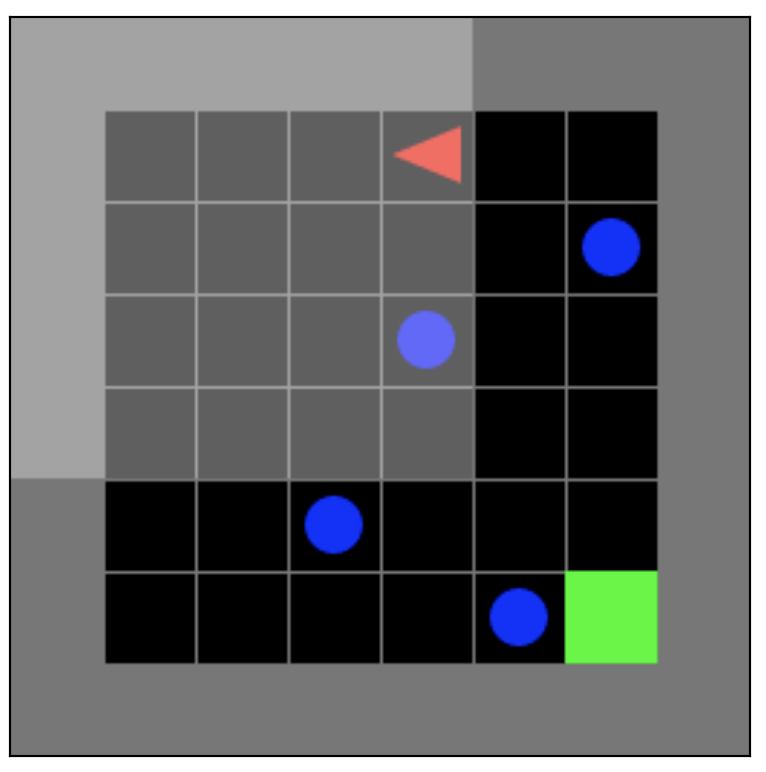
\includegraphics[scale=0.55]{figures/gridworldrl.png}
      \caption{Gridworld with Dynamic Obstacles}
      \label{fig:gridrl}
    \end{figure}
    \columnbreak
    The Reinforcement Learning experiments have been performed on 1M frames for a similar start configuration as shown in \ref{fig:gridrl}. The episode ends when the agent 
    reaches the goal OR collides with an obstacle. We want to encourage the shortest and safest path, thus, the punishment for crashing is $r = -1$. Our rewards are normalized as shown in
    the reward function. We define the range of rewards to be $(-1,1)$. 
\end{multicols}

\subsection{Domain Specific Rules}
The rules are defined as a ProbLog \cite{problog}: a probabilistic prolog that allows us to capture 
the stochasticity of the environment. Precisely, we want to consider the erratic movements of the obstacles, considering 
we do not have previous knowledge on the distribution of their given movement. We assume a uniform distribution and define the following. 
The rules of DIO take the following form: 

\begin{prooftree}
  \AxiomC{$P_0 :: \varphi(0)$}
  \AxiomC{$P_1 :: \varphi(1)$}
  \AxiomC{$P_2 :: \varphi(2)$}
  \AxiomC{$P_3 :: \varphi(3)$}
  \AxiomC{$\ldots$}
  \RightLabel{(action)}
  \QuinaryInfC{$p_1,\ldots, p_n$}
\end{prooftree}
We define $\sum_{i=0}^{n}P(i) = 1$, and $\varphi(i)$ corresponds to the conjunction of grounds facts of the possible world with probability $P_i$.
The action is equivalent to our step semantics, thus, we enforce that a given action modifies the facts in some form. In practice, an action is the missing 
clause to generate the next predicate. In the gridworld example, we give the following. 

\begin{multicols}{2}
\begin{prooftree}
  \AxiomC{atPos(X + V*T, Y)}
  \RightLabel{(right)}
  \LeftLabel{(1)}
  \UnaryInfC{atPos(X,Y), speed(V), timestep(T)}
\end{prooftree}
\columnbreak 
\begin{prooftree}
  \AxiomC{0.25 :: obs(X + V*T, Y, V) \ldots}
  \LeftLabel{(2)}
  \RightLabel{(time)}
  \UnaryInfC{obs(X,Y,V), timestep(T)}
\end{prooftree}
\end{multicols}

(1) considers the movement of the agent while (2) considers the movement of the obstacles. Note that (2) considers 
a uniform distribution over the movement of the obstacle, since every obstacle has a uniform probability of moving up/down/left/right. 
We could do the same for (1) by consider the probability of an action failing. In our case, we assume the movement is deterministic and no failure over the movement 
of the agent happens.


\subsection{World Knowledge}
Our world knowledge base covers the agent, the obstacles and the timestep. We consider two cases: 
\textit{constant} ground facts vs. \textit{dynamic} ground facts. The latter represents positions which are dynamically 
generated at every timestep while the former considers only the facts that remain true in every world, thus include the timestep, since we always
move by 1-unit, and the speed, since the agent and the obtacles are defined to only move by 1-box every time. Given that our knowledge base $Kb$ is defined by, 
\[
    C = \{speed(1), timestep(1) \}     
    \qquad
    D = \{atPos(X, Y), obs(X,Y,1)\}
    \qquad
    Kb = C \cup D
\]

\subsection{From Norms to Labels}
\textcolor{red}{Todo.}

\subsection{Translation Unit}